% in der Präambel (falls noch nicht vorhanden):
% \usepackage{tikz}

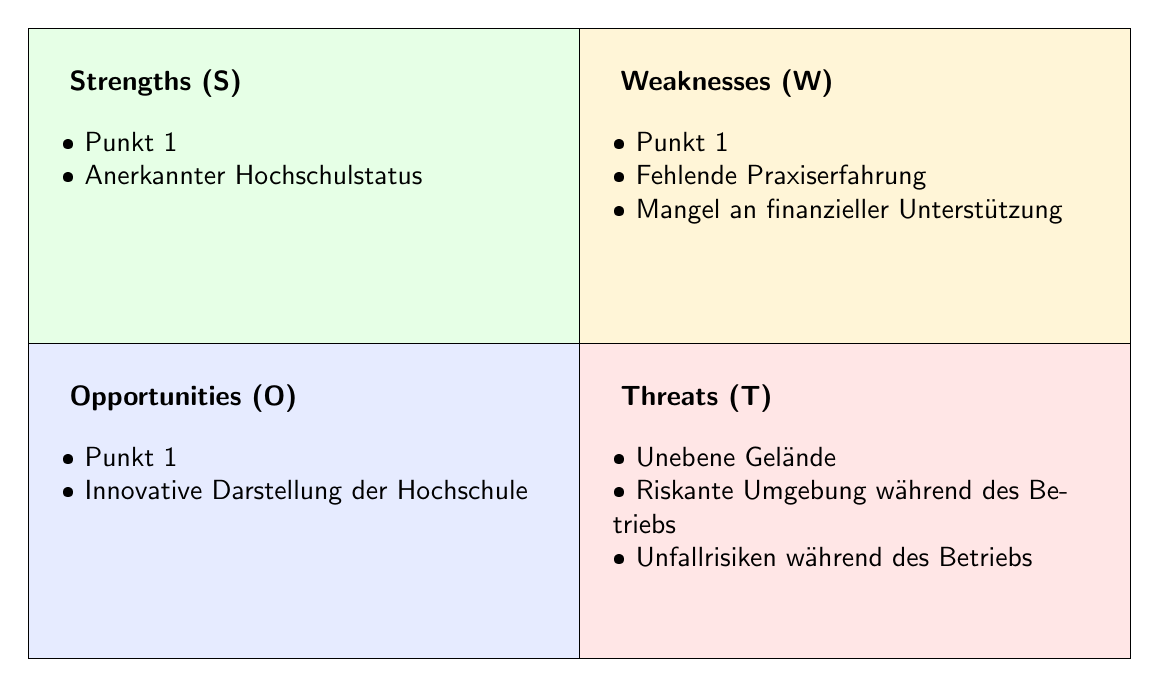
\begin{tikzpicture}[font=\sffamily]
	% Gesamtgröße
	\def\W{14}   % Breite
	\def\H{8}    % Höhe
	
	 % Farben definieren (Pastell)
	\definecolor{swotgreen}{RGB}{230, 255, 230}   % Strengths
	\definecolor{swotorange}{RGB}{255, 245, 215}  % Weaknesses
	\definecolor{swotblue}{RGB}{230, 235, 255}    % Opportunities
	\definecolor{swotred}{RGB}{255, 230, 230}     % Threats
	
	% Hintergrundflächen
	\fill[swotgreen] (0,\H/2) rectangle (\W/2,\H);       % Strengths
	\fill[swotorange] (\W/2,\H/2) rectangle (\W,\H);     % Weaknesses
	\fill[swotblue] (0,0) rectangle (\W/2,\H/2);         % Opportunities
	\fill[swotred] (\W/2,0) rectangle (\W,\H/2);         % Threats
	
	% Rahmen + Unterteilung
	\draw (0,0) rectangle (\W,\H);
	\draw (0,\H/2) -- (\W,\H/2);
	\draw (\W/2,0) -- (\W/2,\H);
	
	% Überschriften (oben links in jedem Feld)
	\node[anchor=north west] at (0.4,\H-0.4) {\textbf{Strengths (S)}};
	\node[anchor=north west] at (\W/2+0.4,\H-0.4) {\textbf{Weaknesses (W)}};
	\node[anchor=north west] at (0.4,\H/2-0.4) {\textbf{Opportunities (O)}};
	\node[anchor=north west] at (\W/2+0.4,\H/2-0.4) {\textbf{Threats (T)}};
	
	% Beispiel-Platzhaltertext (optional – kannst du ersetzen/löschen)
	\node[anchor=north west, align=left, text width=6.3cm] at (0.3,\H-1.2)
	{• Punkt 1\\• Anerkannter Hochschulstatus};
	%{• Punkt 1\\• Punkt 2\\• Punkt 3};
	
	\node[anchor=north west, align=left, text width=6.3cm] at (\W/2+0.3,\H-1.2)
	{• Punkt 1\\• Fehlende Praxiserfahrung\\• Mangel an finanzieller Unterstützung};
	
	\node[anchor=north west, align=left, text width=6.3cm] at (0.3,\H/2-1.2)
	{• Punkt 1\\• Innovative Darstellung der Hochschule};
	
	\node[anchor=north west, align=left, text width=6.3cm] at (\W/2+0.3,\H/2-1.2)
	{• Unebene Gelände\\• Riskante Umgebung während des Betriebs\\• Unfallrisiken während des Betriebs};
\end{tikzpicture}
